\documentclass[dvipdfmx,autodetect-engine,titlepage]{jsarticle}
\usepackage[dvipdfm]{graphicx}
\usepackage{ascmac}
\usepackage{fancybox}
\usepackage{listings}
\usepackage{plistings}
\usepackage{itembkbx}
\usepackage{amsmath}
\usepackage{url}
\usepackage{graphics}
\usepackage{listings}
\usepackage{here}

\lstset{%
  language={C},
  basicstyle={\small},%
  identifierstyle={\small},%
  commentstyle={\small\itshape\color[rgb]{0,0.5,0}},%
  keywordstyle={\small\bfseries\color[rgb]{0,0,1}},%
  ndkeywordstyle={\small},%
  stringstyle={\small\ttfamily\color[rgb]{1,0,1}},
  frame={tb},
  breaklines=true,
  columns=[l]{fullflexible},%
  numbers=left,%
  xrightmargin=0zw,%
  xleftmargin=3zw,%
  numberstyle={\scriptsize},%
  stepnumber=1,
  numbersep=1zw,%
  lineskip=-0.5ex%
}

\textheight=23cm
\renewcommand{\figurename}{図}
\renewcommand{\tablename}{表}
\newenvironment{code}
{\vspace{0.5zw}\VerbatimEnvironment  \begin{screen} 
\baselineskip=1.0\normalbaselineskip
 \begin{Verbatim}}
{\end{Verbatim}
\baselineskip=\normalbaselineskip
 \end{screen}\vspace{0.5zw}} 

\title{セキュリティ・ネットワーク学実験3(B2)\\
インシデント対応演習レポート\\
}
\author{2600200087-2\\Oku Wakana\\奥 若菜}
\date{July 21 2022}

\begin{document}

\maketitle

\section{動作確認}
フォルダSubmitに作った自己紹介ファイルが暗号化されたため、新たにフォルダSubmit2をデスクトップ上に作り、その中に自己紹介ファイルmyfile.odtを作成した。
しばらくすると、下の図1,2のように、Submit2にあったmyfile.odtが、encrypted.zipに暗号化された状態で移動していた。
よって、デスクトップ上に別のフォルダを作成しても、フォルダ内のファイルは同じように暗号化されてしまうことが分かった。\\

\begin{figure}[H]
  \centering
  \begin{minipage}[b]{0.45\linewidth}
  \begin{center}
    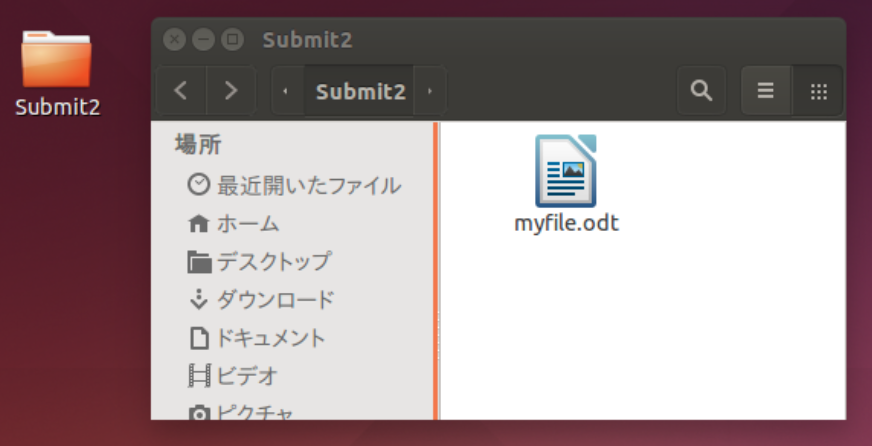
\includegraphics[keepaspectratio,scale=0.46]{in1.png}
    \end{center}
    \caption{Submit2}
  \end{minipage}
  \begin{minipage}[b]{0.45\linewidth}
  \begin{center}
    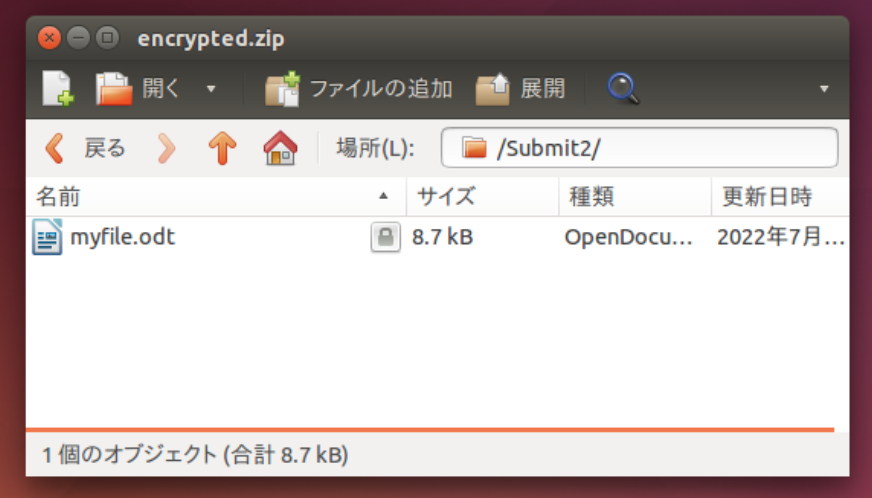
\includegraphics[keepaspectratio,scale=0.44]{in2.png}
    \end{center}
    \caption{encrypted.zip}
  \end{minipage}
\end{figure}

\section{受付番号}
\subsection{チームに割り当てられた仮想マシンの受付番号}
暗号化されたファイルに対して、攻撃者のメッセージが残されており、その中に受付番号が記されていた。
チームに割り当てられたそれぞれの仮想マシンでの受付番号は下の表1のようになった。数の大きさや、どのマシンについても1回目より2回目の方が大きい数になっていることから、受付番号はプロセスID
と関係があるのではないかと考えた。

\begin{table}[H]
  \centering
  \caption{受付番号}
  \begin{tabular}{|c|c|c|}
  \hline
  仮想マシン番号 & 受付番号(1回目) & 受付番号(2回目) \\ \hline
  105   & 2850      & 3171      \\ \hline
  106   & 3389      & 3685      \\ \hline
  109   & 2575      & 2776     \\ \hline
  \end{tabular}
\end{table}
 
\subsection{プロセスログの調査}
受付番号とPIDとの関係を調べるために、仮想マシンに備わっていた「システムログ」というアプリを使用し、プロセスのログを採取した。
下の図3,4はそれぞれ仮想マシン109において、1回目と2回目の暗号化が行われたときのログをキャプチャしたものである。オレンジ色で選択されている部分は、
cronによってコマンドからencrypt.shが実行されたことを記録している。

\begin{figure}[H]
  \centering
  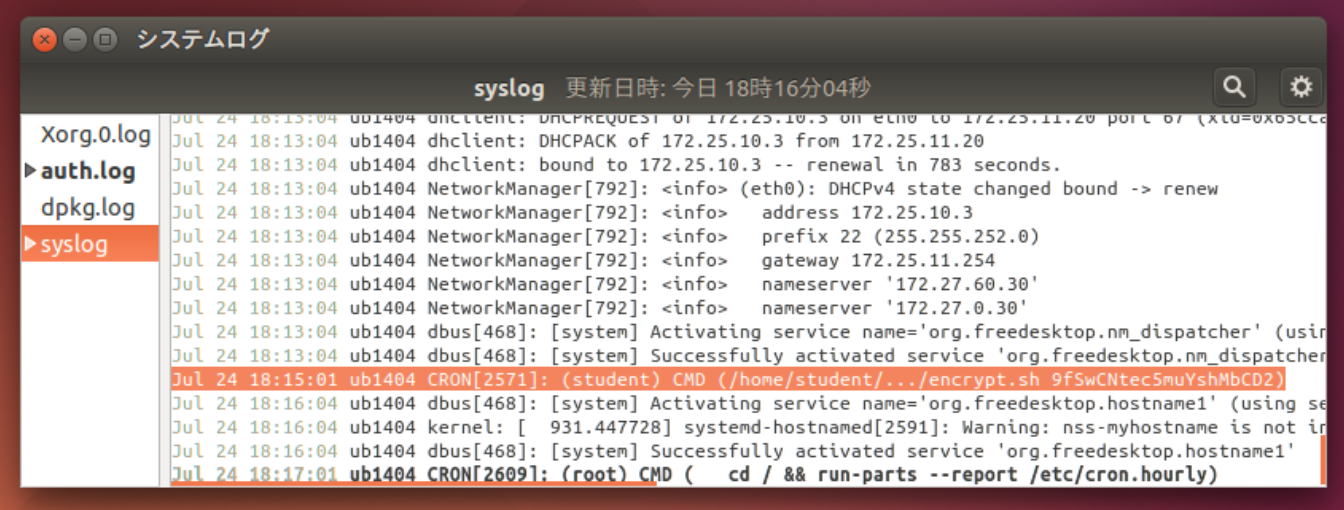
\includegraphics[scale=0.5]{in3.png}
  \caption{1回目のログ}\label{fig:図3}
\end{figure}

\begin{figure}[H]
  \centering
  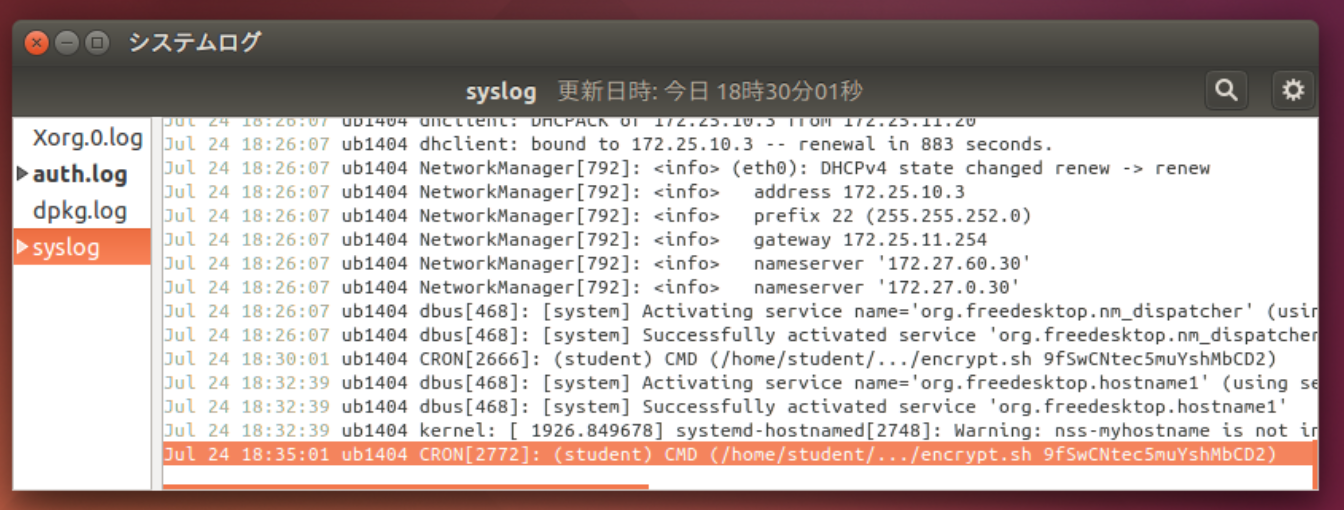
\includegraphics[scale=0.5]{in5.png}
  \caption{2回目のログ}\label{fig:図5}
\end{figure}

 \\
下の表2は、採取したログのcronが実行されたPIDと受付番号を比較したものである。1,2回目どちらも値は一致せず、PIDより受付番号が4つ大きいことが確認できた。
この関係から、受付番号はcronによって実行されたencrypt.shが呼び出したプロセスのPIDであると考えられる。\\
\begin{table}[H]
  \centering
  \caption{cronのPIDと受付番号}
  \begin{tabular}{|c|c|c|}
  \hline
      & cronのPID & 受付番号 \\ \hline
  1回目 & 2571     & 2575 \\ \hline
  2回目 & 2772     & 2776 \\ \hline
  \end{tabular}
\end{table}
 
\subsection{encrypted.shの調査}
2.2章より、受付番号はencrypt.shが呼び出したプロセスのPIDであると考えた。これを確認するために、encrypt.shがどのような動作を行うかを調べる。encrypt.shはhome/...フォルダ上に存在する。
下の図5より、encrypt.shは、デスクトップ上のフォルダ内のファイルを暗号化し、encrypted.zipに移動させ、その後、同じくhome/...フォルダ上にあるhello.shを実行することが分かった。

\begin{figure}[H]
  \centering
  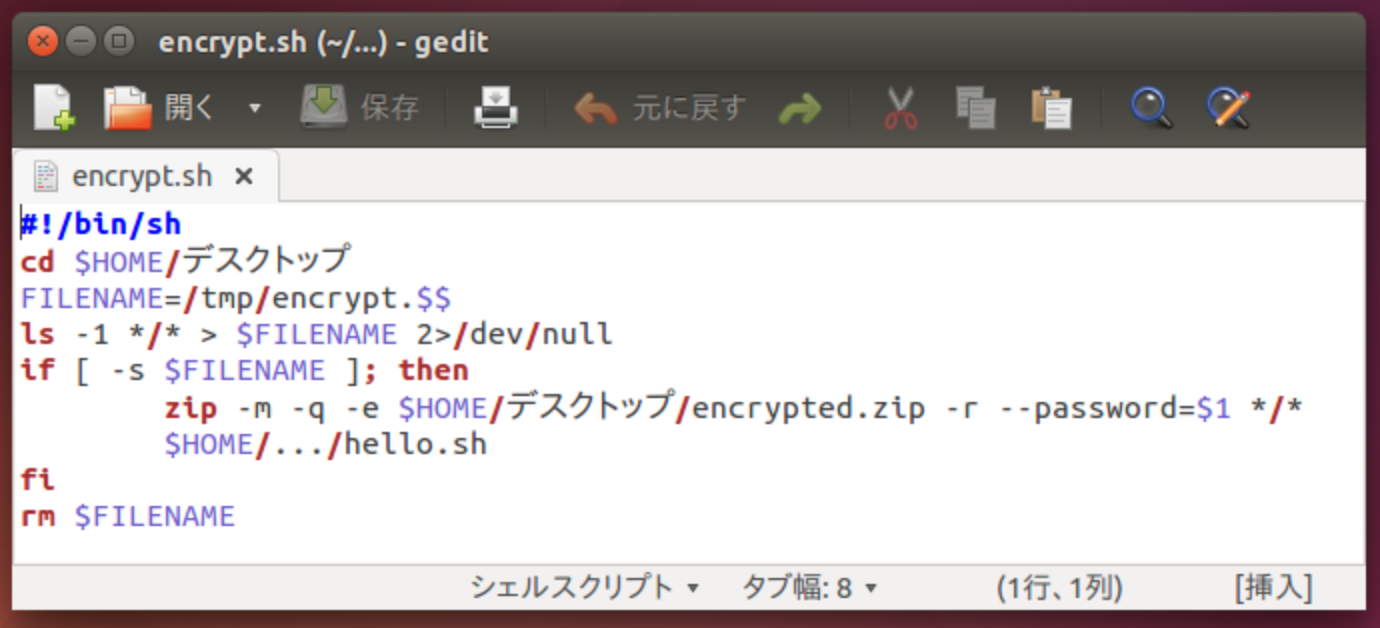
\includegraphics[scale=0.45]{in7.png}
  \caption{encrypt.sh}\label{fig:図7}
\end{figure}

図6より、hello.shの内容から、攻撃者からのメッセージである「大切なお知らせ」はhello.shによって作成されることが分かった。
また、受付番号が\$\$ とされていることから、hollo.shが実行される際のシェルのPIDが、受付番号に用いられていることが確認できた。\\
\begin{figure}[H]
  \centering
  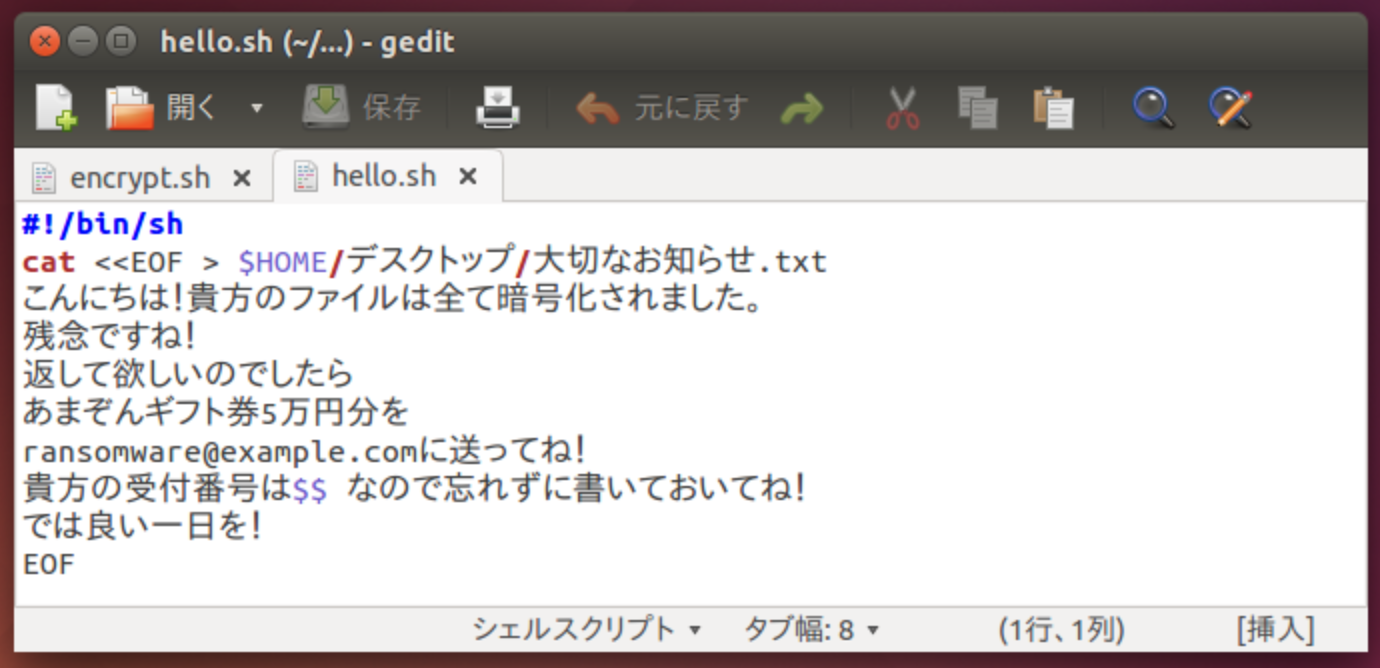
\includegraphics[scale=0.45]{in8.png}
  \caption{hello.sh}\label{fig:図8}
\end{figure}

\section{暗号化されたファイルの復元}
2.3章の図5より、encrypt.shによってzipコマンド実行され、encrypted.zipへの移動とともに、暗号化が行われることが分かった。
このとき、オプションでpasswordが\$1と設定されていることから、暗号化されたファイルを復元するためのパスワードは、encrypt.shを実行するときの第一引数であることが分かる。
図7のように、引数の値はシステムログから確認することができ、これを入力すると暗号化されたファイルを展開することができた。\\
\begin{figure}[H]
  \centering
  \fbox{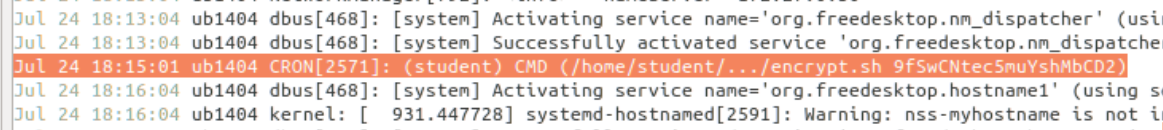
\includegraphics[scale=0.5]{in9.png}}
  \caption{encrypt.shの実行ログ}\label{fig:図9}
\end{figure}

\section{攻撃に使われたプログラム}
ここでは、攻撃に使われた各種プログラムについて、存在する場所、所有者、所有グループ、攻撃に関する役割などをまとめる。下の表3はそれらを示したものである。

  \begin{table}[H]
    \centering
    \caption{攻撃に使われたプログラム}
    \begin{tabular}{|c|c|c|c|c|}
    \hline
    存在する場所                 & プログラム            & 所有者                   & 所有グループ                & 役割                          \\ \hline
                           & encrypt.sh       &                       &                       & 暗号化を行う                      \\ \cline{2-2} \cline{5-5} 
    student/home/.../      & fire\_crontab.sh & www-data              & www-data              & 定期的にencrypt.shを実行する         \\ \cline{2-2} \cline{5-5} 
    \multicolumn{1}{|l|}{} & hello.sh         & \multicolumn{1}{l|}{} & \multicolumn{1}{l|}{} & 攻撃者からのメッセージを作成する            \\ \hline
    student/home/          & .profile         & www-data              & www-data              & ログイン時にfire\_crontab.shを実行する \\ \hline
    var/www/html/          & backdoor.php     & nobody                & nogroup               & 攻撃ファイル受信用Webサーバを立てる            \\ \hline
    usr/etc/               & proftpd.conf     & root                  & root                  & 脆弱性を利用しサーバの作成権限を得る                \\ \hline
    \end{tabular}
  \end{table}
 \\
\section{攻撃の流れ}
\subsection{proftpdの脆弱性}
ここでは、攻撃者によって暗号化が行われるまでの一連の流れをまとめる。
はじめに、攻撃の被害にあった仮想マシンはファイル転送システムにproftpdを使用していた。下の図8から分かるように、proftpdは2014年のものとなっており、これには2015年に見つかったCVE-2015-3306という、リモートから任意のファイルをコピー可能な脆弱性が存在する。
この脆弱性が利用されることで、リモートから任意のコードを実行することも可能である。
図9はproftpd.confの一部であり、サーバーを立てることのできるユーザとグループがそれぞれnobodyとnogroupで設定されていることが分かる。\\\\

\begin{figure}[H]
  \centering
  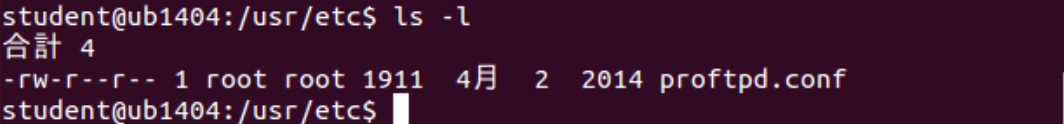
\includegraphics[scale=0.54]{in10.png}
  \caption{proftpdの情報}\label{fig:図10}
\end{figure}

\begin{figure}[H]
  \centering
  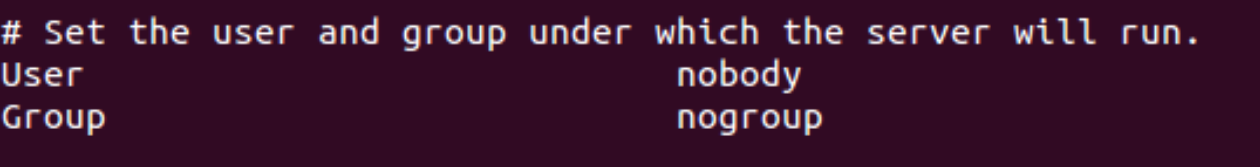
\includegraphics[scale=0.45]{in11.png}
  \caption{proftpdの構成}\label{fig:図11}
\end{figure}

\subsection{仮想マシン内にWebサーバを構築}
proftpdの脆弱性を利用し、攻撃者はnobodyまたはnogroupでログインすることで、仮想マシンにWebサーバを立てることができる。
これにより、var/www/html/にbackdoor.phpが作成された。下の図10はbackdoor.phpの内容であり、このサーバはGETにより受け取った文字列をpassthruでコマンドとして実行する仕様であると分かる。\\

\begin{figure}[H]
  \centering
  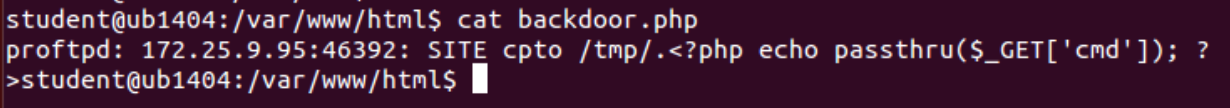
\includegraphics[scale=0.5]{in12.png}
  \caption{backdoor.php}\label{fig:図12}
\end{figure}

\subsection{攻撃用ファイルを転送}
backdoor.phpにより、攻撃者はリモートで任意のコマンドを実行することが可能となった。下の図11はApacheのログであり、攻撃者がbackdoor.phpで構築したWebサーバーにアクセスし、コマンドを実行していることが確認できる。
コマンドの内容としては、攻撃ファイルを自動でダウンロードするWebサイト\url{http://uso.pyon.com/sh.tgz}にアクセスを行ったり、.profileを書き換え、ログイン時にfire\_crontab.shを実行するようなものがある。\\
\begin{figure}[H]
  \centering
  \fbox{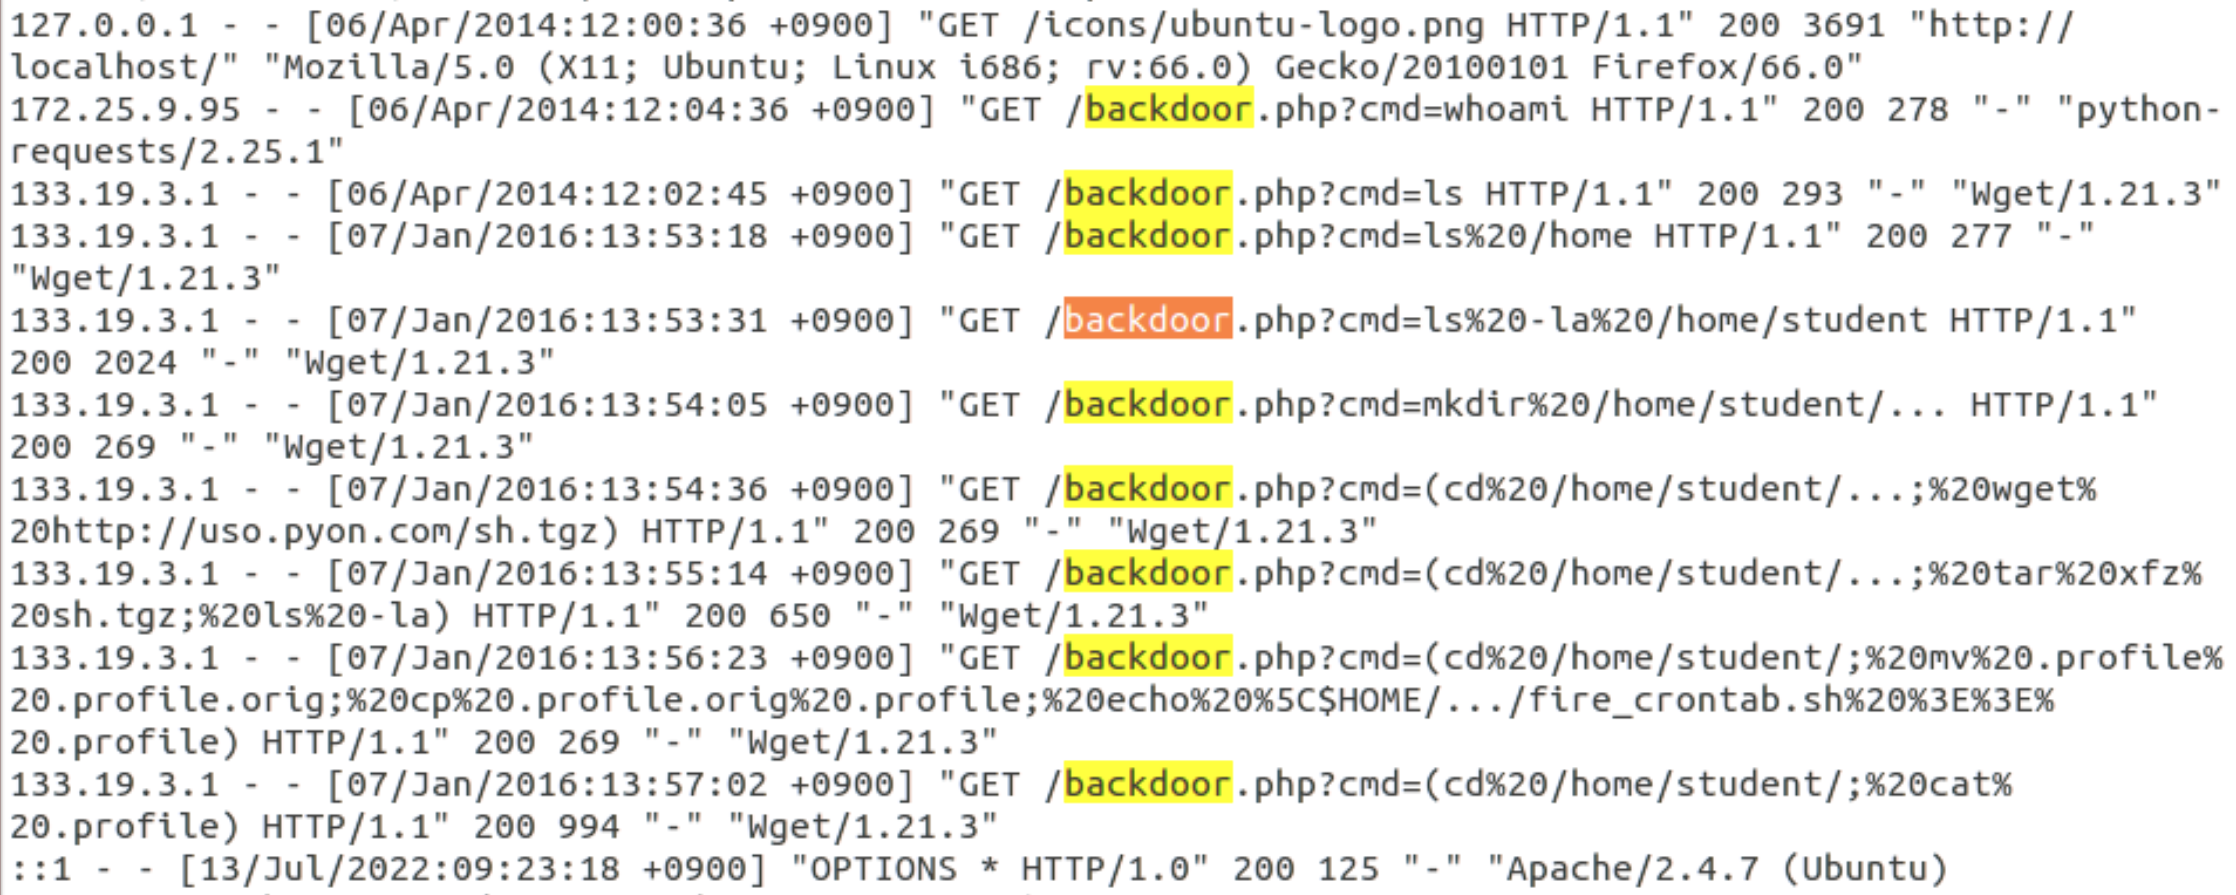
\includegraphics[scale=0.4]{in13.png}}
  \caption{Apacheのログ}\label{fig:図13}
\end{figure}

\subsection{攻撃用ファイルが自動で起動}
student/home/...に存在したencrypt.shなどのシェルスクリプトは、上記の方法で仮想マシンにダウンロードされていた。
また、.profileが書き換えられたことで、ログイン時に自動でfire\_crontab.shが実行されるようになっている。
これによって、encrypt.shが5分毎に実行され、暗号化が自動で行われる。

\end{document}
